\documentclass[a4paper]{article}
\usepackage[left=3cm,right=3cm,top=2cm,bottom=2cm]{geometry} % page settings
\usepackage{enumerate}
\usepackage{hyperref}
\usepackage{graphicx}
\usepackage{amsfonts}
\usepackage{amsthm}
\usepackage{mathtools}
\usepackage{titlesec}
\usepackage{polski}
\usepackage{tikz}
\usepackage[utf8]{inputenc}
\DeclarePairedDelimiter\ceil{\lceil}{\rceil}
\DeclarePairedDelimiter\floor{\lfloor}{\rfloor}

\def\checkmark{\tikz\fill[scale=0.3](0,.35) -- (.25,0) -- (1,.7) -- (.25,.15) -- cycle;} 

\titlespacing*{\subsection}
{0ex}{10ex}{3ex}

\title{Lista 14}
\author{Kamil Matuszewski}
\date{29 stycznia 2016}

\begin{document}

\maketitle
\setlength{\parindent}{0.5ex}
\setlength{\parskip}{1.5ex}
\newcommand{\R}{\mathbb{R}}

\begin{center}
\begin{tabular}{|c *{8}{|c} |c|}\hline
1 & 2 & 3 & 4 & 5 & 6 & 7 & 8 & 9\\
\hline 
\checkmark &\checkmark &\checkmark &\checkmark &\checkmark &\checkmark &\checkmark &\checkmark & \\
\hline
\end{tabular}\\
\end{center}

\subsection*{Zadanie 1}
Oblicz wektory reszt $\widetilde{r}=A\widetilde{x} + b$ $\widehat{r}=A\widehat{x}+b$ oraz wektory błędów $\widetilde{e}=x-\widetilde{x}$ $\widehat{e}=x-\widehat{x}$ dla:

$$A=\begin{vmatrix}
780 & 563\\
913 & 659
\end{vmatrix},
b=\begin{vmatrix}
217\\
254
\end{vmatrix},
\widetilde{x}=\begin{vmatrix}
0.999\\
-1.001
\end{vmatrix},
\widehat{x}=\begin{vmatrix}
0.341\\
-0.087
\end{vmatrix}
$$


$$A\widetilde{x} =\begin{vmatrix}
215.657\\
252.428
\end{vmatrix}$$

$$A\widehat{x} =\begin{vmatrix}
216.999\\
254
\end{vmatrix}$$

$$A\widetilde{x}-b =
\begin{vmatrix}
-1.343\\
-1.572
\end{vmatrix}$$

$$A\widehat{x}-b =
\begin{vmatrix}
-0.001\\
0
\end{vmatrix}$$

$$x =
\begin{vmatrix}
 1\\
-1
\end{vmatrix}
$$
$$\widetilde{e} =
\begin{vmatrix}
-0.001\\
-0.001
\end{vmatrix}
$$
$$\widehat{e} =
\begin{vmatrix}
-0.659\\
0.913
\end{vmatrix}$$

\clearpage
\subsection*{Zadanie 2}
Znajdź rozkład macierzy 
$$A=\begin{vmatrix}
1 & 2 & 3 & 4\\
2 & 9 & 12 & 15\\
3 & 26 & 41 & 49\\
5 & 40 & 107 & 135
\end{vmatrix}$$

Potem wykorzystaj ten rozkład do obliczenia wartości jej wyznacznika oraz macierzy $A^{-1}$

Wystarczy rozwiązać układ równań:\\
$$u_{ij} = a_{ij} - \sum\limits_{k=1}^{i-1} l_{ik}u_{kj}$$
$$l_{ji} = \frac{1}{u_{ii}} (a_{ji}- \sum\limits_{k=1}^{i-1} l_{jk}u_{ki})$$

$L=\begin{vmatrix}
1 & 0 & 0 & 0\\
2 & 1 & 0 & 0\\
3 & 4 & 1 & 0\\
5 & 6 & 7 & 1
\end{vmatrix}$

$U=\begin{vmatrix}
1 & 2 & 3 & 4\\
0 & 5 & 6 & 7\\
0 & 0 & 8 & 9\\
0 & 0 & 0 & 10
\end{vmatrix}$

$$det(A)=det(L)\cdot det(U) = 1\cdot det(U) = det(U)=400 $$

Żeby policzyć $A^{-1}$ wystarczy policzyć $U^{-1}\cdot L^{-1}$.
$$[U|I]=\begin{vmatrix}
1 & 2 & 3 & 4\\
0 & 5 & 6 & 7\\
0 & 0 & 8 & 9\\
0 & 0 & 0 & 10
\end{vmatrix}\begin{vmatrix}
1 & 0 & 0 & 0\\
0 & 1 & 0 & 0\\
0 & 0 & 1 & 0\\
0 & 0 & 0 & 1
\end{vmatrix} \rightarrow \begin{vmatrix}
1 & 0 & 0 & 0\\\\
0 & 1 & 0 & 0\\\\
0 & 0 & 1 & 0\\\\
0 & 0 & 0 & 1
\end{vmatrix}\begin{vmatrix}
1 &	\frac{-2}{5} &	\frac{-3}{40} &	\frac{-21}{760}\\\\
0 &	 \frac{1}{5} &	\frac{-3}{20} &	 \frac{-1}{380}\\\\
0 &	   0 &	  \frac{1}{8} &	 \frac{-9}{152}\\\\
0 &	   0 &	    0 &	   \frac{1}{19}

\end{vmatrix}$$ 
$$[L|I]=\begin{vmatrix}
1 & 0 & 0 & 0\\ 
2 & 1 & 0 & 0\\
3 & 4 & 1 & 0\\
5 & 6 & 7 & 1\\
\end{vmatrix}\begin{vmatrix}
1 & 0 & 0 & 0\\
0 & 1 & 0 & 0\\
0 & 0 & 1 & 0\\
0 & 0 & 0 & 1
\end{vmatrix} \rightarrow \begin{vmatrix}
1 & 0 & 0 & 0\\
0 & 1 & 0 & 0\\
0 & 0 & 1 & 0\\
0 & 0 & 0 & 1
\end{vmatrix}\begin{vmatrix}
  1	& 0 & 0 & 0\\
 -2 & 1 & 0 & 0\\
  5 & -4 & 1 & 0\\
-28 & 22 & -7 & 1
\end{vmatrix}$$ 

Teraz wystarczy wymnożyć:\\
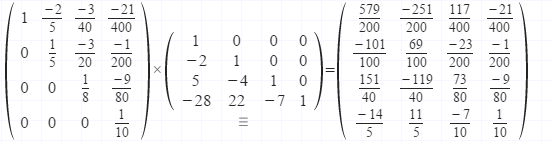
\includegraphics[scale=0.5]{1.png}\\
Można sprawdzić, że działa:\\

\includegraphics[scale=0.5]{2.png}


\clearpage
\subsection*{Zadanie 3}
Stosując metodę faktoryzacji, rozwiąż układ równań:

$$A=\begin{vmatrix}
1 & 1 & 1 & 1\\
1 & 3 & 3 & 3\\
1 & 3 & 6 & 6\\
1 & 3 & 6 & 8
\end{vmatrix}$$

$$B=\begin{vmatrix}
4\\
10\\
16\\
18
\end{vmatrix}$$



Najpierw, podobnie jak w poprzednim, rozbijam macierz A na L i U:
$$A=LU$$
$$L=\begin{vmatrix}
1 & 0 & 0 & 0\\
1 & 1 & 0 & 0\\
1 & 1 & 1 & 0\\
1 & 1 & 1 & 1
\end{vmatrix}$$
$$U=\begin{vmatrix}
1 & 1 & 1 & 1\\
0 & 2 & 2 & 2\\
0 & 0 & 3 & 3\\
0 & 0 & 0 & 2
\end{vmatrix} $$

Teraz policzę $Ly=b$ i $Ux=y$ 
$$\begin{vmatrix}
1 & 0 & 0 & 0\\
1 & 1 & 0 & 0\\
1 & 1 & 1 & 0\\
1 & 1 & 1 & 1
\end{vmatrix} \cdot \begin{vmatrix}
y_1 \\ y_2 \\ y_3 \\ y_4
\end{vmatrix}=\begin{vmatrix}
4 \\ 10 \\ 16 \\ 18
\end{vmatrix}$$
$$\begin{vmatrix}
y_1 \\ y_2 \\ y_3 \\ y_4
\end{vmatrix} = \begin{vmatrix}
4 \\ 6 \\ 6 \\ 2
\end{vmatrix} $$
$$\begin{vmatrix}
1 & 0 & 0 & 0\\
1 & 1 & 0 & 0\\
1 & 1 & 1 & 0\\
1 & 1 & 1 & 1
\end{vmatrix} \cdot \begin{vmatrix}
x_1 \\ x_2 \\ x_3 \\ x_4
\end{vmatrix}=\begin{vmatrix}
4 \\ 6 \\ 6 \\ 2
\end{vmatrix}$$

$$\begin{vmatrix}
x_1 \\ x_2 \\ x_3 \\ x_4
\end{vmatrix} = \begin{vmatrix}
1 \\ 1 \\ 1 \\ 1
\end{vmatrix} $$

\subsection*{Zadanie 4}
Opracuj algorytm znajdowania rozkładu LU macierzy trójprzekątniowej.

Mając macierz
$$\begin{vmatrix}
b_1 & c_1&&&0\\
a_2 & b_2 & c_2\\
& \ddots & \ddots & \ddots\\
&& a_{n-1} &b_{n-1} &c_{n-1}\\
0&&& a_n &b_n
\end{vmatrix} = \begin{vmatrix}
1 & 0&&&0\\
l_2 & 1 & 0\\
& \ddots & \ddots & \ddots\\
&& l_{n-1} &1 &0\\
0&&& l_n &1
\end{vmatrix}
\begin{vmatrix}
u_1 & d_1&&&0\\
0 & u_2 & d_2\\
& \ddots & \ddots & \ddots\\
&& 0 &u_{n-1} &d_{n-1}\\
0&&& 0 &u_n
\end{vmatrix}$$

Teraz, z mnożenia macierzy $A=LU$:
$$d_k=c_k$$
$$b_1=u_1 \Rightarrow u_1=b_1 $$
$$a_k=l_ku_{k-1} \Rightarrow l_k=\frac{a_k}{u_{k-1}}$$
$$b_k=l_kc_{k-1}+u_k \Rightarrow u_k=b_k-l_kc_{k-1} $$

\subsection*{Zadanie 5}
(a)
Pokaż, że iloczyn dwóch macierzy dolnotrójkątnych (górno) jest macierzą dolnotrójkątną (górno).
\begin{proof}

Niech $C=AB$. $C=(c_{ij})$, gdzie:
$$c_{ij}=\sum\limits_{s=1}^n a_{is}b_{sj}.$$
Ustalmy $i<j$, ponieważ B jest trójkątna dolna, dla $s<j$ $b_{sj}=0$, więc:
$$c_{ij}=\sum\limits_{s=j}^n a_{is}b_{sj}.$$
Ale A też jest trójkątna dolna, więc dla $i<s$ $a_{is}=0$, co daje nam $c_{ij}=0$ dla $i<j$.\\
Analogicznie dla trójkątnej górnej.

\end{proof}
(b)
Pokaż, że jeśli A jest macierzą trójkątną dolną z jedynkami na głównej przekątnej, to sama jest macierzą tego typu.

\begin{proof}

Używając metody Gaussa-Jordana wychodzimy od macierzy $[I|A]$ wystarczy odpowiednio wyeliminować kolejne kolumny macierzy A. W ten sposób nie naruszymy ani głównej przekątnej ani miejsc nad główną przekątną. W końcu powstanie nam macierz $[B|I]$, gdzie B jest macierzą dolnotrójkątną z jedynkami na głównej przekątnej. Wiemy, że macierz B jest macierzą odwrotną do A.

\end{proof}
\subsection*{Zadanie 6}
Zaproponuj algorytm wyznaczania macierzy odwrotnej do macierzy dolnotrójkątnej i oszacuj jego złożoność.

Metoda eliminacji Gaussa-Jordana. Wykonujemy kolejno (n-1) odejmowań (do eliminowania pierwszej kolumny), (n-2) (do drugiej kolumny), (n-3), \dots , (n-n+1), (n-n).\\
Daje nam to sumaryczną złożoność $O(n^2)$. Nie miała być turboszybka xD


\clearpage
\subsection*{Zadanie 7}
Metodą eliminacji w wersji skalarnej rozwiąż układ równań:

$$\left\{ \begin{matrix}
3x_1 & + & 4x_2 & + & 3x_3 & = & 16\\
x_1 & + & 5x_2 & - & x_3 & = & -12\\
6x_1 & + & 3x_2 & + & 7x_3 & = & 102\\
\end{matrix}\right. $$

$$\left\{ \begin{matrix}
3x_1 & + & 4x_2 & + & 3x_3 & = & 16\\
0 & + & \frac{11}{3}x_2 & - & 2x_3 & = & \frac{-52}{3}\\
0 & - & 5x_2 & + & x_3 & = & 70\\
\end{matrix}\right. $$

$$\left\{ \begin{matrix}
3x_1 & + & 4x_2 & + & 3x_3 & = & 16\\
0 & + & \frac{11}{3}x_2 & - & 2x_3 & = & \frac{-52}{3}\\
0 & + & 0 & - & \frac{19}{11} & = \frac{510}{11}\\
\end{matrix}\right. $$


$$x=\begin{vmatrix}
58\\ \\
-\frac{368}{19}\\ \\
-\frac{510}{19}
\end{vmatrix}$$

\clearpage
\subsection*{Zadanie 8}
Rozwiąż układ z poprzedniego zadania stosując metodę macierzową.

$$A=\begin{vmatrix}
3 & 4 & 3\\
1 & 5 & -1\\
6 & 3 & 7\\
\end{vmatrix}$$

$$M^{(1)}=\begin{vmatrix}
1 & 0 & 0 \\
-\frac{1}{3}  & 1 & 0 \\
-2 & 0 & 1
\end{vmatrix}$$

$$A^{(2)}=M^{(1)}A^{(1)}=
\begin{vmatrix}
3 && 4 && 3\\ \\
0 && \frac{11}{3} && -2\\ \\
0 && -\frac{15}{3} && 1\\ \\
\end{vmatrix}$$

$$b^{(2)}=M^{(1)}b^{(1)}=\begin{vmatrix}
16\\
-\frac{52}{3}\\
70
\end{vmatrix}$$

$$M^{(2)}=\begin{vmatrix}
1 & 0 & 0 \\
0  & 1 & 0 \\
0 & \frac{15}{11} & 1
\end{vmatrix}$$

$$A^{(3)}=M^{(2)}A^{(2)}=
\begin{vmatrix}
3 && 4 && 3\\ \\
0 && \frac{11}{3} && -2\\ \\
0 && 0 && -\frac{30}{11}\\ \\
\end{vmatrix}$$

$$b^{(3)}=M^{(2)}b^{(2)}=\begin{vmatrix}
16\\ \\
-\frac{52}{3}\\ \\
\frac{510}{11}
\end{vmatrix}$$

$$x=\begin{vmatrix}
58\\ \\
-\frac{368}{19}\\ \\
-\frac{510}{19}
\end{vmatrix}$$


\end{document}